% ===============================================================
%  CHAPITRE 1 — MÉTHODE (~6 pages)
% ===============================================================
\chapter[Méthode]{Reconstruire heure par heure un territoire sans mesure horaire}
\label{chap:methode}

\section{Démarche d'ensemble et indicateurs}
\label{sec:demarche}

Aucune courbe de charge publique n'existe à la maille d'une intercommunalité. Les gestionnaires de réseau publient en revanche des volumes annuels locaux et des profils horaires régionaux, tandis que d'autres organismes décrivent la météo, la population, le parc automobile ou le foncier. Notre méthode consiste à assembler ces sources pour reconstruire, pour chaque heure de 2021 à 2025, la consommation et la production des Mauges, puis à simuler sur ces séries les scénarios demandés. La figure~\ref{fig:chaine} résume cette chaîne, dont chaque maillon est détaillé dans la suite du chapitre.

\begin{figure}[H]
\centering
\begin{tikzpicture}[
  box/.style={draw=esieeBlue, fill=LightGray, rounded corners=3pt, align=center, font=\footnotesize, minimum height=1.25cm, text width=2.45cm},
  dark/.style={box, fill=esieeBlue, text=white},
  arr/.style={-{Stealth[length=2.5mm]}, thick, color=esieeBlue!70}]
\node[box] (d) {Données publiques\\ électriques, météo,\\ INSEE, réseau, foncier};
\node[box, right=0.45cm of d] (t) {Collecte, traçabilité\\ et harmonisation\\ à l'heure};
\node[box, right=0.45cm of t] (r) {Reconstruction\\ horaire de la\\ consommation et\\ de la production};
\node[box, right=0.45cm of r] (m) {Moteur de bilan\\ horaire, 5 années\\ météo};
\node[dark, right=0.45cm of m] (s) {Indicateurs\\ et simulateur};
\draw[arr] (d) -- (t); \draw[arr] (t) -- (r); \draw[arr] (r) -- (m); \draw[arr] (m) -- (s);
\node[font=\scriptsize\itshape, color=accentOrange, below=0.15cm of t, text width=2.6cm, align=center] {contrôles automatiques};
\node[font=\scriptsize\itshape, color=accentOrange, below=0.15cm of r, text width=2.6cm, align=center] {corrections et\\ recalages};
\node[font=\scriptsize\itshape, color=accentOrange, below=0.15cm of m, text width=2.6cm, align=center] {bilans fermés\\ à chaque heure};
\end{tikzpicture}
\caption{Chaîne de traitement, des données publiques au simulateur}
\label{fig:chaine}
\end{figure}

Les indicateurs sont ceux de la fiche du projet, à savoir l'énergie produite, le taux de couverture, le surplus, le déficit et la pointe d'injection. Leur définition mérite toutefois d'être précisée, car deux \og taux de couverture \fg{} coexistent. Le premier rapporte la production annuelle à la consommation annuelle et ne mesure qu'un volume. Le second, que nous retenons, mesure la part de la consommation réellement satisfaite par la production locale au moment où elle a lieu. En notant $P_h$ la production et $C_h$ la consommation de l'heure $h$, il s'écrit
\begin{equation}
\tau = \frac{\sum_h \min(P_h,\, C_h)}{\sum_h C_h},
\label{eq:couverture}
\end{equation}
la batterie, lorsqu'elle existe, modifiant $P_h$ par ses charges et ses décharges. La fiche ne définit pas précisément l'écrêtement. Nous l'avons interprété comme l'énergie produite au-delà du seuil de vigilance, c'est-à-dire au-delà de $1{,}2\,C_h$, exprimée en pourcentage de la production annuelle. Ce choix relie les deux règles de la fiche et revient à considérer qu'au-delà de 120~\% de la consommation locale, l'injection supplémentaire n'est plus acceptée par le réseau. Enfin, nous exigeons que la limite de 5~\% soit respectée pour chacune des cinq années météo étudiées et pas seulement en moyenne, afin qu'une année ensoleillée ne suffise pas à rendre une trajectoire non conforme.

\section{Comprendre le territoire avant de le modéliser}
\label{sec:territoire}

Avant de calculer, nous avons cherché à comprendre qui consomme dans les Mauges et pourquoi. Cette étape n'est pas décorative. Elle conditionne plusieurs hypothèses du modèle et fournit des ordres de grandeur pour juger de la cohérence des résultats. Les données de l'\gls{insee}~\cite{insee_dossier}, comparées au Maine-et-Loire, à la région et à la France, dessinent un territoire très particulier (figure~\ref{fig:territoire}).

\begin{figure}[H]
\centering
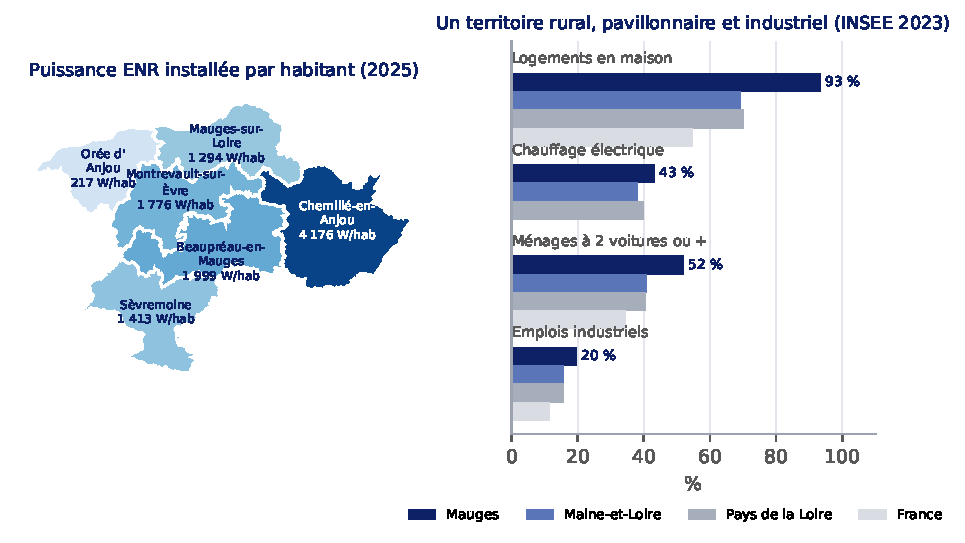
\includegraphics[width=\textwidth]{territoire.pdf}
\caption{Répartition de la puissance renouvelable installée et profil socio-économique des Mauges~\cite{odre_registre, insee_dossier}}
\label{fig:territoire}
\end{figure}

Les Mauges sont d'abord un territoire pavillonnaire. 93~\% des logements sont des maisons, contre 55~\% en France, et 43~\% des résidences principales sont chauffées à l'électricité. Il n'est donc pas surprenant qu'un habitant y consomme 2~455~kWh par an pour son logement en 2023, soit 20~\% de plus que la moyenne française, ni qu'un logement y consomme 5,5~MWh contre 4,1 en moyenne nationale~\cite{enedis_secteur}. C'est ensuite un territoire industriel et agricole, puisque 20~\% des emplois relèvent de l'industrie et 10~\% de l'agriculture, soit presque deux fois et quatre fois la moyenne nationale. L'agroalimentaire représente à lui seul plus du tiers de la consommation industrielle mesurée par Enedis. C'est enfin un territoire où la voiture est indispensable. 52~\% des ménages possèdent au moins deux voitures, contre 35~\% en France, alors que les véhicules électriques ne représentent encore que 2,4~\% du parc en 2025~\cite{sdes_ve}.

Ces constats ont trois conséquences directes sur la modélisation. La forte part de chauffage électrique rend la consommation résidentielle sensible au froid, ce qui justifie de travailler sur plusieurs années météo. Le poids de l'industrie impose de traiter à part les sites raccordés directement au réseau de transport, dont la consommation ne suit pas les saisons (section~\ref{sec:conso}). Enfin, le nombre de ballons d'eau chaude électriques et de véhicules, qui détermine le potentiel des flexibilités étudiées, est estimé à partir de ces données démographiques et non posé arbitrairement.

La carte de la figure~\ref{fig:territoire} soulève une autre question, celle de l'équité territoriale. La puissance renouvelable installée varie de 218~W par habitant à Orée d'Anjou à 4~176~W par habitant à Chemillé-en-Anjou, qui accueille l'essentiel de l'éolien. Une trajectoire de développement ne se juge donc pas seulement sur ses indicateurs globaux. Elle se juge aussi sur la répartition de ses impacts entre les communes, question que nous retrouverons lors de l'étude du réseau.

\section{Choix, collecte et traitement des données}
\label{sec:donnees}

Le tableau~\ref{tab:sources} présente les familles de données mobilisées et l'usage qui en est fait. Nous avons volontairement dépassé les seules données électriques. La météo sert à corriger la production, les données démographiques à dimensionner les usages, les données de réseau à localiser les raccordements et les données foncières à vérifier que la surface ne constitue pas une contrainte.

\begin{table}[H]
\centering
\footnotesize
\caption{Principales sources de données et usage dans l'étude}
\label{tab:sources}
{\renewcommand{\arraystretch}{1.2}
\begin{tabularx}{\textwidth}{@{}>{\raggedright\arraybackslash}p{2.1cm}>{\raggedright\arraybackslash}X>{\raggedright\arraybackslash}p{2.9cm}>{\raggedright\arraybackslash}X@{}}
\toprule
\textbf{Famille} & \textbf{Données} & \textbf{Source} & \textbf{Usage} \\
\midrule
Production & Parc par installation ; production régionale horaire & \gls{odre}~\cite{odre_registre}, \gls{rte}~\cite{rte_eco2mix}, Enedis~\cite{enedis_agregats} & Puissances des scénarios, facteurs de charge \\
Consommation & Volume annuel de l'\gls{epci} par secteur ; profils horaires & \gls{odre}~\cite{odre_conso}, Enedis~\cite{enedis_secteur}, éCO2mix & Courbe de charge locale \\
Météo & Rayonnement, vent, température horaires & Météo-France~\cite{meteofrance} & Corrections de production, \gls{dju} \\
Territoire & Population, logements, chauffage, projections & \gls{insee}~\cite{insee_dossier, insee_omphale} & Ballons, horizon 2035, contrôles \\
Mobilité & Véhicules par commune et type de recharge & \gls{sdes}~\cite{sdes_ve} & Parc de \gls{ve} en 2035 \\
Réseau & Capacité \gls{s3renr} des postes sources ; quote-part & Caparéseau~\cite{capareseau}, DREAL~\cite{dreal_s3renr} & Lieux et coût de raccordement \\
Foncier & Toitures, parkings, zones au sol favorables & \gls{cerema}, IGN~\cite{cerema_pv} & Surface exploitable en solaire \\
Économie & Coût des batteries, tarifs, objectifs locaux & \gls{nrel}~\cite{nrel2025}, \gls{cre}~\cite{cre_trve}, \gls{pcaet}~\cite{pcaet} & \gls{van}, objectifs du territoire \\
\bottomrule
\end{tabularx}}
\end{table}

Les données ont été collectées par les interfaces de programmation d'ODRÉ et d'Enedis ou par export direct, soit 46 téléchargements. Chacun est consigné dans un manifeste qui conserve l'adresse exacte de la requête, la date et l'empreinte du fichier, de sorte que toute la chaîne peut être rejouée. Les séries ont ensuite été harmonisées. Les données au pas de 30~minutes ont été ramenées à l'heure, toutes les dates exprimées en \gls{utc} pour éviter les doublons du changement d'heure, et les unités converties en MW et MWh. Les trous de deux heures au plus ont été comblés par interpolation linéaire et signalés, ce qui concerne 2,4~\% des heures, principalement en 2024 et 2025. Les trous plus longs ont été laissés vides. Un script de contrôle vérifie enfin à chaque relance les bilans, les bornes physiques et l'absence de valeurs aberrantes.

Ces contrôles ont permis de détecter plusieurs incohérences avant qu'elles ne contaminent les résultats. Enedis indique par exemple pour 2022 des degrés-jours inférieurs de 41~\% à ceux de 2021, alors que nos degrés-jours recalculés à partir de la station Météo-France de Saint-Florent-le-Vieil ne baissent que de 16 à 22~\% selon la convention retenue. Pour toutes les autres années, nos calculs encadrent pourtant ceux d'Enedis. Nous avons donc écarté la valeur 2022 publiée. De même, en 2024, ODRÉ classe 130~GWh en \og non affecté \fg{} et retire autant de l'industrie, ce qui nous a conduits à calculer la répartition sectorielle sur la période 2021-2023.

\section{Reconstruire la consommation horaire}
\label{sec:conso}

La consommation horaire des Mauges est obtenue en répartissant le volume annuel mesuré selon une forme horaire régionale. L'hypothèse sous-jacente est qu'à l'intérieur d'un même secteur, un logement ou une usine des Mauges consomme au même rythme que son homologue régional. Le volume local capte donc le poids propre du territoire, tandis que la forme régionale apporte la météo de l'année et les cycles journaliers et hebdomadaires. Deux variantes ont été construites. La méthode S applique à chaque secteur le profil Enedis correspondant, disponible pour 2024 et 2025. La méthode R utilise la consommation régionale publiée par éCO2mix, disponible sur les cinq années. La figure~\ref{fig:conso} montre qu'elles sont très proches. Sur 2024, leur corrélation horaire atteint 0,97, la pointe diffère de 2,8~\% et l'écrêtement du scénario B de 0,2 point seulement. Nous avons donc retenu la méthode R pour les cinq années.

\begin{figure}[H]
\centering
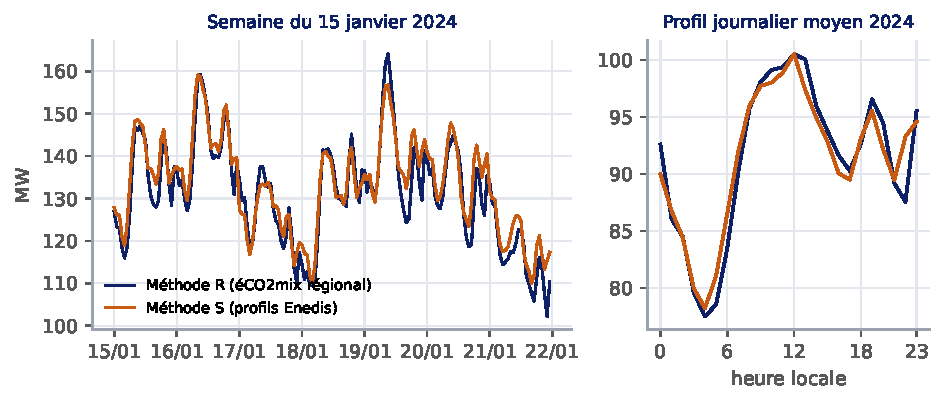
\includegraphics[width=\textwidth]{conso_methodes.pdf}
\caption{Comparaison des deux méthodes de reconstruction de la consommation (2024)}
\label{fig:conso}
\end{figure}

Deux corrections complètent cette reconstruction. La consommation de 2025 n'étant pas encore publiée, nous l'avons estimée en appliquant au volume de 2024 l'évolution de la consommation régionale entre 2024 et 2025, et signalée comme telle. Surtout, l'écart entre la consommation totale publiée par ODRÉ et la somme des consommations communales d'Enedis représente chaque année entre 14,5 et 16,6~\% du total. Cet écart correspond aux sites raccordés directement au réseau de transport, essentiellement industriels, ce que confirme le fait qu'il se retrouve presque entièrement dans le secteur industriel. Or la consommation nationale de ces clients ne présente pratiquement aucune saisonnalité, avec un rapport hiver sur été de 0,96 contre 1,47 pour la consommation totale. Appliquer à cette part le profil régional, très marqué par le chauffage, aurait donc surestimé les pointes d'hiver. Nous l'avons modélisée par un profil plat, ce qui réduit la pointe de soutirage d'environ 8~\%.

\section{Reconstruire la production horaire}
\label{sec:prod}

La production horaire est obtenue en multipliant la puissance installée dans les Mauges par le facteur de charge régional de chaque heure, publié par éCO2mix pour le solaire et l'éolien. Les autres filières, bioénergie et hydraulique, représentent moins de 2~\% de la production et sont considérées comme constantes. Le même parc, celui du 31 décembre 2025, est appliqué aux cinq années afin de ne faire varier que la météo. Cette construction simple a cependant révélé deux biais qu'il a fallu corriger.

Le premier vient d'éCO2mix lui-même. Le facteur de charge publié est le rapport entre la production et une capacité installée qui n'est mise à jour que par paliers. Entre deux mises à jour, le parc réel continue de croître alors que le dénominateur reste figé, si bien que le facteur de charge dérive à la hausse puis chute brutalement. Ainsi, la capacité solaire régionale reste fixée à 1~212~MW de décembre 2023 à novembre 2024 avant de bondir à 1~642~MW (figure~\ref{fig:capacite}). Nous avons reconstruit une capacité lissée par interpolation linéaire entre les paliers, en considérant que chaque palier publié correspond au parc réel à sa date. Le facteur de charge solaire de 2024 passe alors de 13,8 à 11,6~\%, ce qui fait de 2024 l'année la moins ensoleillée de la période. Ce résultat est cohérent avec le rayonnement mesuré à Beaucouzé, qui est lui aussi le plus faible en 2024.

\begin{figure}[H]
\centering
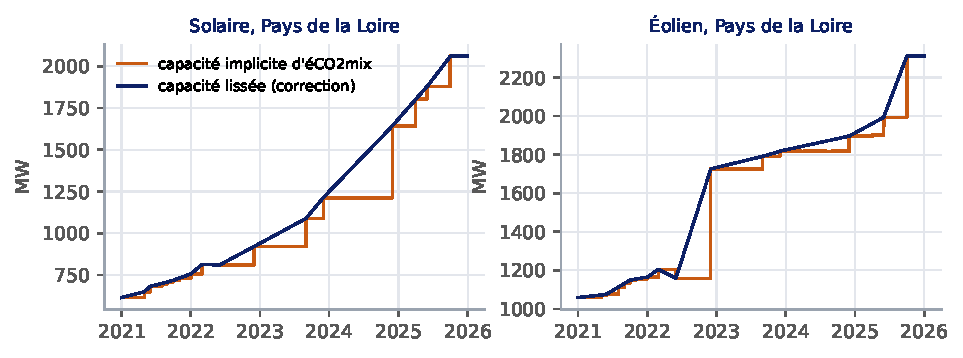
\includegraphics[width=\textwidth]{capacite_eco2mix.pdf}
\caption{Capacité installée implicite d'éCO2mix et capacité lissée retenue}
\label{fig:capacite}
\end{figure}

Le second biais concerne l'éolien. Depuis la mise en service du parc en mer de Saint-Nazaire fin 2022, le profil régional mêle production en mer et production terrestre, alors que les Mauges n'ont que des éoliennes terrestres. À vent égal mesuré à Cholet, le facteur de charge régional augmente de 6 à 17~\% après cette date. Nous avons donc corrigé le niveau annuel de l'éolien à vent égal, année par année. Pour vérifier que la forme horaire n'était pas elle aussi biaisée, nous l'avons remplacée en 2024 et 2025 par celle de la production éolienne d'Enedis, qui ne concerne que des parcs terrestres. Le taux de couverture varie de moins d'un point, ce qui nous a conduits à conserver la forme éCO2mix, seule disponible sur toute la période.

Enfin, les productions simulées ont été recalées sur la production réellement injectée par les installations des Mauges, issue du registre national. Les coefficients obtenus valent 0,900 pour le solaire et 0,859 pour l'éolien, les installations locales produisant un peu moins que la moyenne régionale. Cette étape répond aussi à une question posée par la fiche, qui impose 15~\% de pertes photovoltaïques. Notre production étant calée sur des mesures réelles, ces pertes y sont déjà incluses, et les appliquer une seconde fois reviendrait à les compter deux fois.

\section{Moteur de simulation, hypothèses et validation}
\label{sec:moteur}

Le moteur calcule pour chaque heure le bilan entre production et consommation, puis les indicateurs de la section~\ref{sec:demarche}. La batterie de la fiche a une puissance égale à la puissance solaire du scénario, une durée de deux heures et un rendement aller-retour de 90~\%. Deux pilotages ont été comparés. Le premier stocke tout surplus dès que la production dépasse la consommation, ce qui maximise la couverture mais remplit souvent la batterie avant le pic de midi. Le second ne stocke que l'énergie qui dépasse le seuil de 120~\%, afin de garder sa capacité pour éviter l'écrêtement. Trois autres leviers ont été modélisés, à savoir le déplacement vers la mi-journée de la chauffe des ballons d'eau chaude, le pilotage de la recharge des \gls{ve} et un plafond d'injection des installations solaires. Un horizon 2035 intègre enfin l'électrification des usages à partir des hypothèses des fiches des projets 1 et 3 et des projections de l'\gls{insee}, avec 25~\% des logements équipés d'une \gls{pac} et 40~\% de véhicules électriques~\cite{fiche_projets, insee_omphale, rte_bp2025}. L'ensemble des hypothèses et de leurs sources figure en annexe~\ref{annexe:hypotheses}.

Le volet économique repose sur la \gls{van} sur 15 ans, actualisée à 4~\% selon le taux retenu par \gls{rte}~\cite{rte_fe2050}.
\begin{equation}
\mathrm{VAN} = -I + \sum_{t=1}^{15} \frac{G - C_{\mathrm{OM}}}{(1+0{,}04)^{t}},
\label{eq:van}
\end{equation}
où $I$ est l'investissement, $G$ le gain annuel et $C_{\mathrm{OM}}$ le coût annuel d'exploitation. Les coûts proviennent des projections du \gls{nrel} pour 2025, soit 395~€ par kWh de capacité et 49~€ par kW et par an d'exploitation~\cite{nrel2025, bce}. Le gain correspond à l'électricité qui n'est plus achetée au réseau, valorisée au tarif réglementé de 0,194~€/kWh~\cite{cre_trve}, diminuée du surplus qui n'est plus vendu à 0,02~€/kWh~\cite{cre_surplus}.

Les résultats sont donnés en moyenne sur 2021-2025 avec la fourchette des cinq années. L'année 2022, la plus proche de la moyenne sur l'ensemble des indicateurs, sert d'année type pour les représentations heure par heure. Un modèle peut tourner sans erreur et rester faux, c'est pourquoi nous avons vérifié le moteur par des propriétés physiques. À chaque heure, la consommation doit se répartir exactement entre production locale, décharge de la batterie et achats au réseau, et la production entre consommation directe, charge et export, faute de quoi le calcul s'arrête. Le scénario A sert aussi de témoin, puisque sa couverture horaire doit rester proche de sa couverture en volume (section~\ref{sec:actuel}), et les principaux ordres de grandeur se recalculent à la main (annexe~\ref{annexe:calculs}). Le simulateur, accessible à l'adresse \lienSimulateur, repose sur ce même moteur. Il permet de faire varier chaque hypothèse et propose une vue destinée aux élus, une vue de démonstration et une vue experte (figure~\ref{fig:simulateur}).

\begin{figure}[H]
\centering
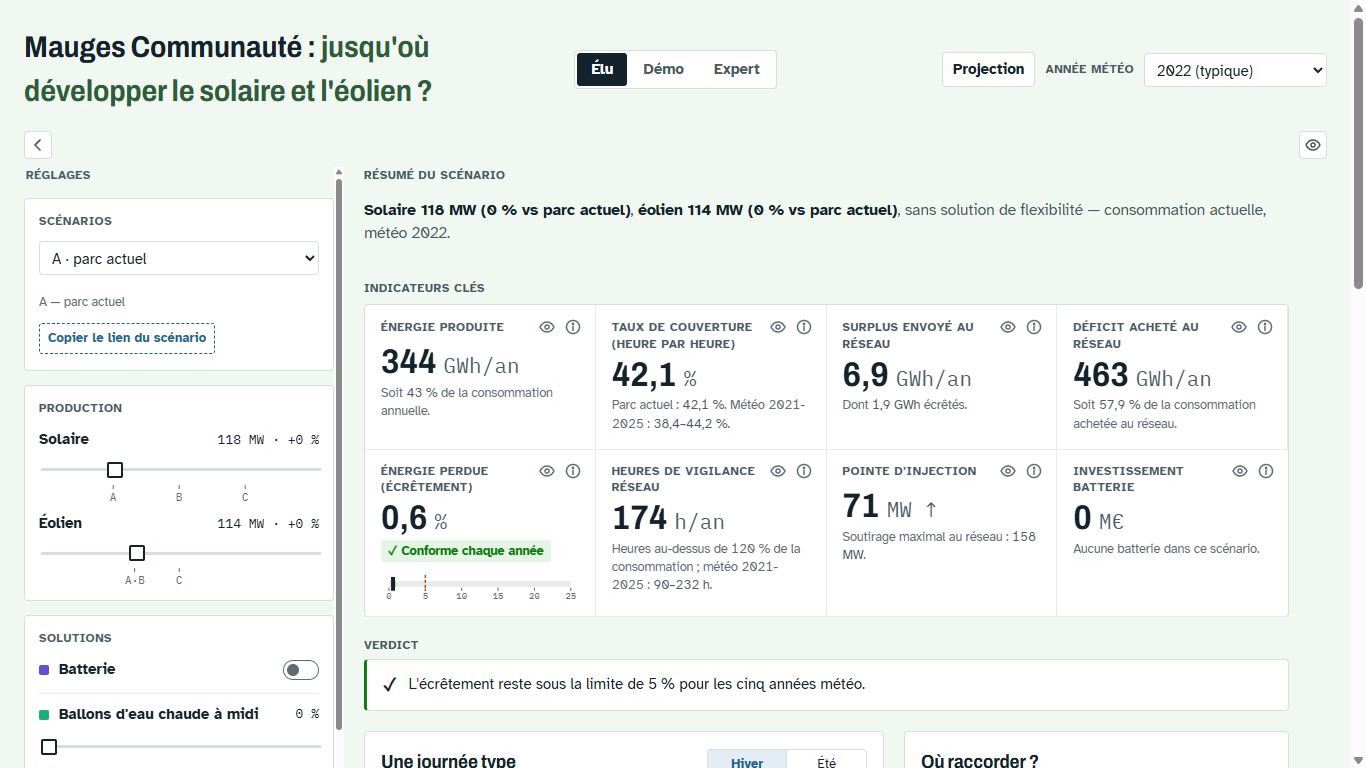
\includegraphics[width=0.82\textwidth]{simulateur_elu.png}
\caption{Vue Élu du simulateur, scénario A, année météo 2022}
\label{fig:simulateur}
\end{figure}
